\documentclass[conference]{IEEEtran}
\usepackage{cite}
\usepackage{amsmath,amssymb}
\usepackage{graphicx}
\usepackage{pgfplots}
\usepgfplotslibrary{groupplots}
\usetikzlibrary{arrows.meta,positioning}
\pgfplotsset{compat=1.18}
\definecolor{auditblue}{RGB}{33,113,181}
\definecolor{auditorange}{RGB}{179,88,6}
\usepackage{booktabs,array}
\usepackage[hidelinks]{hyperref}
\usepackage[capitalise,nameinlink]{cleveref}
\crefname{figure}{Fig.}{Figs.}
\crefname{table}{Table}{Tables}
\graphicspath{{figures/}}
\newcolumntype{L}[1]{>{\raggedright\arraybackslash}p{#1}}
\newcommand{\cwruShapRuntime}{0.57--1.04}
\newcommand{\cwruHardware}{Apple M3}
\newcommand{\cwruShapVersion}{0.52.0}

\newcommand{\dtuModelRuntime}{16.9}
\newcommand{\dtuSourceRuntime}{594}

\raggedbottom
\begin{document}
\title{Reference Design for Mechanism-Level SHAP Audits in Predictive Maintenance}
\author{\IEEEauthorblockN{Koshik Debanath, Prakrit Uprety, Vision Rijal, and Peiyu Li}
\IEEEauthorblockA{Department of Computer Science, South Dakota State University, Brookings, SD, USA\\
koshik.debanath@jacks.sdstate.edu, prakrit.uprety@jacks.sdstate.edu,\\
vision.rijal@jacks.sdstate.edu, peiyu.li@sdstate.edu}}
\hypersetup{pdftitle={Reference Design for Mechanism-Level SHAP Audits in Predictive Maintenance},pdfauthor={Koshik Debanath, Prakrit Uprety, Vision Rijal, Peiyu Li},pdfsubject={Reference transfer, context-shift harm, and mechanism-level attribution audits},pdfkeywords={SHAP, explanation evaluation, conformal calibration, distribution shift, predictive maintenance, bearing diagnosis}}
\maketitle
\begin{abstract}
Mechanism-level SHAP audits compare feature attributions with an expected failure-mechanism map. We examine whether their warnings transfer beyond the function used for calibration and whether they identify harmful context dependence. A perfect-predictor example first shows that genuine overlap produces outside-set attribution. Across 1,200 learned reference--candidate pairs, thresholds with approximately 5\% warning rates on the reference warn on independently fitted, decision-equivalent models at rates up to 14.1\%. Calibration over independent aligned fits broadens the statistical target to a specified training population, but does not certify arbitrary acceptable models. When a formerly reliable context input becomes independent, mean F1 losses range from 0.121 to 0.390 at 10,000 rows per batch, yet SHAP-excess localization on harm-positive models falls to zero. A prediction-response baseline retains sensitivity at matched empirical acceptable-model warning rates. A prospective continuous-process study calibrates on 100 independently seeded model/run-packet pairs. SHAP gives 0/60 warnings on unaltered evaluation pairs and localizes a constructed acquisition bias in 60/60 pairs; removing that bias lowers mean F1 from 0.965 to 0.665. Measured bearing and mill studies expose incomplete mechanism maps and missing comparison cohorts. These results distinguish reference-relative deviation, input reliance, transfer harm, and comparison support before an explanation warning informs maintenance decisions.
\end{abstract}
\begin{IEEEkeywords}
SHAP, explanation evaluation, conformal calibration, distribution shift, predictive maintenance
\end{IEEEkeywords}

\section{Introduction}
\label{sec:introduction}
\subsection{Problem Statement}
An explanation for a maintenance prediction should help an engineer decide what to inspect. A classifier may rely on an acquisition condition associated with a fault instead of a signature that transfers across equipment~\cite{geirhos2020shortcut,lapuschkin2019unmasking}. Feature attribution describes the fitted prediction, but an audit needs an additional decision: which attribution patterns justify a warning?

A common starting point is a map from a recorded failure mechanism to expected features. Attribution outside that map may indicate an unintended association, an incomplete map, or another genuine mechanism occurring in the same rows. A redundant measurement creates a further ambiguity: using it may be harmless while its association remains stable and harmful when that association changes. These cases require different evidence.

\subsection{Research Objective}
We ask whether warnings transfer between aligned fits, whether localization detects harmful reliance, and whether SHAP improves sensitivity over direct response. Rank validity and engineering usefulness are separate questions.

Our controlled study makes the mechanism map and full model response observable. We compare independently trained acceptable models, stable surrogates, and fixed candidates exposed to weakening or reversed context associations. A continuous-process experiment tests prospective calibration over independently seeded fits and whole-run packets. Bearing and mill studies assess attribution under a constructed acquisition response and the availability of mechanism-comparison cohorts.

\subsection{Contributions}
The contributions are:
\begin{itemize}
\item A reference-design analysis distinguishing a fixed-function null from a population of aligned training outcomes, with an exact overlap counterexample and explicit unit requirements.
\item A paired evaluation of reference transfer, harm-defined context shifts, direct non-SHAP baselines, and source-derived overlap bins. The evaluation exposes both excess warnings on acceptable models and missed harmful dependence.
\item A prospective continuous-process audit with a non-SHAP comparator, complemented by measured vibration audits and explicit calibration/data budgets.
\end{itemize}
Conformal ranks and overlap stratification are existing tools. Our contribution is the paired measurement of warnings on acceptable refits and harm-conditional localization under explicit calibration populations.

\section{Related Work and Background}
\label{sec:background}
\subsection{Explanation Evaluation and Testing}
SHAP assigns feature contributions to a fitted prediction~\cite{lundberg2017shap}. The choice between interventional and observational value functions changes what the explanation represents~\cite{chen2020true,sundararajan2020many,janzing2020feature}. Neither choice turns attribution into a physical-cause estimate~\cite{kumar2020problems}. Our expected-feature share is related to relevance mass accuracy~\cite{arras2022clevr}; synthetic relevance benchmarks and OpenXAI provide other controlled evaluation settings~\cite{liu2021synthetic,agarwal2022openxai}.

Permutation importance~\cite{altmann2010permutation}, conditional randomization~\cite{candes2018panning}, SHAP-XRT~\cite{teneggi2023shapxrt}, and population Shapley importance~\cite{williamson2020shapley} address reliance or importance through different null hypotheses. SHAP-XRT tests a local conditional-independence target; we test batch-level excess relative to a supplied mechanism map and reference law. Our finite-difference baseline is a direct response comparison, not an implementation of SHAP-XRT or a conditional randomization test. Explanation methods may also miss spurious reliance~\cite{adebayo2022spurious} or be manipulated~\cite{slack2020fooling}. Explanation Shift compares explanation distributions across domains~\cite{mougan2025shift}; our shift experiment instead asks whether a mechanism-specific localization event coincides with measured predictive harm.

Neuhaus et al.~\cite{neuhaus2023spurious} validate harmful image shortcuts using images containing a suspected feature without the class object. Our intervention holds mechanism counts fixed while changing context association. Their neural image-concept pipeline is not a baseline for our supplied Boolean response tables, but their distinction between correlated and harmful features motivates evaluating predictive consequences rather than input use alone.

\subsection{Conformal References}
Split-conformal ranks provide marginal control under exchangeability~\cite{angelopoulos2023conformal}. Mondrian methods condition calibration on categories~\cite{vovk2005algorithmic,vovk2012conditional}; conditional conformal methods extend the range of conditional targets~\cite{gibbs2025conditional}, and weighted methods address specified covariate shifts~\cite{tibshirani2019shift}. These results motivate stratification, not a new calibration theorem. We compare fixed overlap bins with bins learned from source covariates, and distinguish marginal control from calibration-conditional uncertainty~\cite{vovk2012conditional,bates2023outliers}.

\subsection{Bearing Diagnosis}
Maintenance-XAI work motivates mechanism-informed inspection~\cite{matzka2020explainable,vollert2021interpretable}. CWRU benchmarking studies document difficult fault signatures and dependence between operating conditions~\cite{smith2015cwru,hendriks2022benchmarking}. Loads from the same damaged bearing do not provide independent new-bearing tests. We therefore use diameter holdout and retain entire recordings. The task is fault-location diagnosis from vibration-derived features, with no healthy-bearing class.

Field measurements introduce a separate annotation question. Lundstr\"om and O'Nils~\cite{lundstrom2023factory} describe eleven mill cases with manual spectral labels and inspection when available; mixed faults receive the most distinct class. Such labels support diagnosis studies but do not supply an exhaustive feature-relevance map. Adding field data therefore does not by itself establish physical alignment or sufficient independent calibration units.

\subsection{Problem Definition and SHAP}
\Cref{tab:notation} fixes the terminology. For a scalar model output $h(x)$ and feature subset $J$, our interventional value function is
\begin{equation}
 v_h(J;x)=\mathbb E_{X'\sim\widehat P}[h(x_J,X'_{-J})].
 \label{eq:background}
\end{equation}
The selected inputs come from $x$; missing inputs come jointly from one background row. For $d$ inputs, the attribution is
\begin{align}
 \phi_j^h(x)&=\sum_{J\subseteq[d]\setminus\{j\}}w_d(J)\,\Delta_j^h(J;x),\label{eq:shap}\\
 \Delta_j^h(J;x)&=v_h(J\cup\{j\};x)-v_h(J;x),\\
 w_d(J)&=\frac{|J|!(d-|J|-1)!}{d!}.
\end{align}
The coefficient averages the prediction change from adding feature $j$ over feature orders. In the Boolean study, $d=4$ and the empirical audit batch is the background, so all states and subsets are enumerated. The measured study uses interventional TreeSHAP with training-only backgrounds.

\begin{table}[t]
\centering
\caption{Terms used throughout the audit. A reference may be a fixed function or a specified distribution of independently trained functions.}
\label{tab:notation}
\footnotesize
\begin{tabular}{L{0.14\columnwidth}L{0.76\columnwidth}}
\toprule
Symbol & Meaning \\
\midrule
$f$, $g$, $h$ & Reference predictor, candidate predictor, and a generic scalar predictor \\
$E_m$ & Expected features supplied for mechanism $m$ \\
$\mathcal I_m$, $\mathcal F$ & Rows with mechanism $m$; all recorded failure rows \\
$C$ & A supplied context input; use alone does not establish harm \\
$A_h$, $L_h$ & Maximum excess; excess localizing the specified context \\
Aligned fit & Mechanism-only model meeting the stated full-state gate \\
Harm-positive & Candidate with mean F1 loss at least 0.05 under independent context \\
\bottomrule
\end{tabular}
\end{table}

\subsection{Audit Statistics}
For a nonempty row group $A$, define mean absolute attribution and normalized share as
\begin{equation}
 a_j^h(A)=\frac{1}{|A|}\sum_{x\in A}|\phi_j^h(x)|,
 \qquad s_j^h(A)=\frac{a_j^h(A)}{\sum_k a_k^h(A)}.
\end{equation}
The normalization is a ratio of group means, not a mean of per-row ratios. Omitting superscript $h$ when the model is clear, relevant share, specificity, and outside-set excess are
\begin{align}
 R_m&=\sum_{j\in E_m}s_j(\mathcal I_m),\\
 D_m&=R_m-\sum_{j\in E_m}s_j(\mathcal F\setminus\mathcal I_m),\\
 S_m&=\max_{j\notin E_m}\{s_j(\mathcal I_m)-s_j(\mathcal F\setminus\mathcal I_m)\}.
 \label{eq:outside}
\end{align}
$R_m$ measures correspondence to expected features. $D_m$ measures whether that correspondence is stronger on own-mechanism rows. $S_m$ selects the outside feature with the greatest increase in share. Empty groups or zero attribution make the statistic unavailable.

Let $A_h(X)=\max_m S_m^h(X)$ for batch $X$. For localization, retain $S_m^h$ only when its maximizing outside feature is $C$, then maximize over those mechanisms; call the result $L_h(X)$, or $-\infty$ if none qualifies. Ties use a fixed feature order. Localization is an attribution event pointing to $C$, not a finding of transfer harm.

\subsection{Mechanism Overlap}
An exact example shows why an outside feature need not be suspect. Let $Z_0=Z_1\sim\operatorname{Bernoulli}(\pi)$ and independent $Z_2\sim\operatorname{Bernoulli}(\rho)$, with perfect predictor $h_\lor=Z_0\lor Z_1\lor Z_2$ and $E_m=\{Z_m\}$. Interventional Shapley values retain dependence among missing inputs. On mechanism-0 rows, exact enumeration gives
\begin{align}
 a_0(\mathcal I_0)=a_1(\mathcal I_0)&=(1-\pi)(1-\rho)/2,\\
 a_2(\mathcal I_0)&=2\rho(1-\pi)(1-\rho)/3.
\end{align}
Other failure rows have $Z_0=Z_1=0,Z_2=1$, where
\begin{align}
 a_0=a_1&=\pi(1-\rho)/6,\\
 a_2&=(1-\rho)(3-2\pi)/3.
\end{align}
Normalizing yields
\begin{equation}
 s_1(\mathcal I_0)=\frac{3}{6+4\rho},\qquad
 s_1(\mathcal F\setminus\mathcal I_0)=\frac{\pi}{6-2\pi}.
\end{equation}
At $\pi=\rho=0.05$, $S_0=0.4754$, maximized by genuine mechanism $Z_1$. This is established credit sharing under dependence~\cite{janzing2020feature,kumar2020problems}; the example identifies its consequence for the warning score. It does not imply that an unlisted redundant input is harmful.

\section{Methodology}
\label{sec:method}
\subsection{Reference Choice and Audit Procedure}
Specify the prediction, expected map, comparison cohort, and intended decision; keep acquisitions grouped. \Cref{tab:reference-scope,fig:workflow} guide reference choice and computation. For physical claims, distinguish supported, causally excluded, and unresolved features. Missing graph paths and non-rejections remain unresolved~\cite{gamella2025chamber}. $S_m$ measures deviation from the supplied map; a causal-exclusion warning would instead require separately validated excluded features. An empty excluded set or unsupported calibration population requires abstention from that claim.

\begin{table*}[t]
\centering
\caption{Reference scope. Nineteen independent units give finite 5\% rank resolution, not useful precision. Model draws are separate training outcomes.}
\label{tab:reference-scope}
\footnotesize
\begin{tabular}{L{0.18\textwidth}L{0.28\textwidth}L{0.23\textwidth}L{0.21\textwidth}}
\toprule
Reference/check & Supported statement & Required units & Scope \\
\midrule
Expected-set comparison & Attribution corresponds to the supplied map and cohort & Defined groups and nonzero attribution & Descriptive $R_m,D_m,S_m$ \\
Fixed-function rank & Warning on a new batch from the reference's score law & At least 19 per base bin and 19 target-calibration batches & One fixed $f$; not another acceptable fit \\
Training-population rank & Warning on a new eligible fit and batch from the same procedure & One batch per independent fit; at least 19 scores per bin & Specified training law and eligibility gate \\
Targeted response test & Prediction changes when the known context input is flipped & Defined intervention and calibration ranks & Input reliance; does not establish transfer harm \\
\bottomrule
\end{tabular}
\end{table*}

\begin{figure*}[t]
\centering
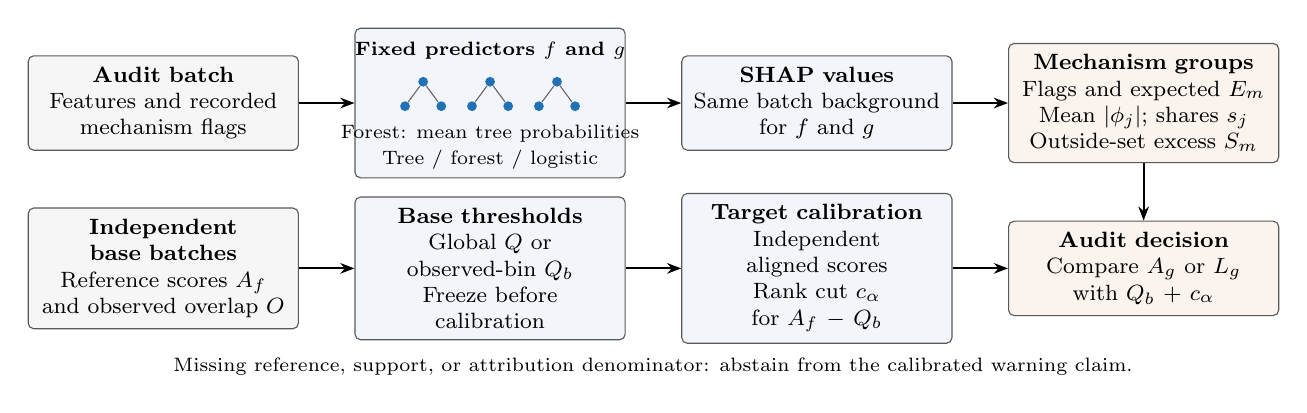
\begin{tikzpicture}[
  font=\footnotesize,
  block/.style={draw=black!65,rounded corners=2pt,align=center,text width=3.15cm,minimum height=1.05cm,inner sep=4pt},
  link/.style={-{Stealth[length=1.8mm]},line width=0.7pt},
  hint/.style={font=\scriptsize,align=center},
  dot/.style={circle,fill=auditblue,inner sep=1.25pt}]
\node[block,fill=gray!7] (data) at (0,0) {\textbf{Audit batch}\\Features and recorded\\mechanism flags};
\node[block,fill=auditblue!6,minimum height=1.9cm] (model) at (4.15,0) {};
\node[hint] at (4.15,0.66) {\textbf{Fixed predictors $f$ and $g$}};
\foreach \x [count=\i] in {3.30,4.15,5.00} {
  \node[dot] (root\i) at (\x,0.27) {};
  \node[dot] (left\i) at (\x-0.23,-0.04) {};
  \node[dot] (right\i) at (\x+0.23,-0.04) {};
  \draw[black!60] (root\i)--(left\i) (root\i)--(right\i);
}
\node[hint] at (4.15,-0.39) {Forest: mean tree probabilities};
\node[hint] at (4.15,-0.72) {Tree / forest / logistic};
\node[block,fill=auditblue!6] (shap) at (8.30,0) {\textbf{SHAP values}\\Same batch background\\for $f$ and $g$};
\node[block,fill=auditorange!7] (scores) at (12.45,0) {\textbf{Mechanism groups}\\Flags and expected $E_m$\\Mean $|\phi_j|$; shares $s_j$\\Outside-set excess $S_m$};
\node[block,fill=gray!7] (base) at (0,-2.10) {\textbf{Independent base batches}\\Reference scores $A_f$\\and observed overlap $O$};
\node[block,fill=auditblue!6] (bins) at (4.15,-2.10) {\textbf{Base thresholds}\\Global $Q$ or observed-bin $Q_b$\\Freeze before calibration};
\node[block,fill=auditblue!6] (cal) at (8.30,-2.10) {\textbf{Target calibration}\\Independent aligned scores\\Rank cut $c_\alpha$ for $A_f-Q_b$};
\node[block,fill=auditorange!7] (decision) at (12.45,-2.10) {\textbf{Audit decision}\\Compare $A_g$ or $L_g$\\with $Q_b+c_\alpha$};
\draw[link] (data)--(model);
\draw[link] (model)--(shap);
\draw[link] (shap)--(scores);
\draw[link] (base)--(bins);
\draw[link] (bins)--(cal);
\draw[link] (cal)--(decision);
\draw[link] (scores)--(decision);
\node[hint] at (6.22,-3.35) {Missing reference, support, or attribution denominator: abstain from the calibrated warning claim.};
\end{tikzpicture}

\caption{Fixed-function audit with a common batch background and independent base/target-calibration batches. Population calibration instead uses one score per independent training draw.}
\label{fig:workflow}
\end{figure*}

\subsection{Fixed-Function Calibration}
Mechanism flags provide observed overlap
\begin{equation}
 O(X)=\frac{\sum_i\mathbf1\{Z_{0i}=1,Z_{1i}=1\}}{\sum_i\mathbf1\{Z_{0i}=1\}}.
\end{equation}
A base bank supplies global $Q$ or overlap-bin $Q_b$. We compare fixed bins $[0,0.8),[0.8,0.9),[0.9,1]$ with source-only tertiles/quintiles, estimated from 1000 source batches per fixed function or one source batch per calibration fit. Fixed edges exploit the designed target law.

Freeze the base reference and define residual score
\begin{equation}
 T_h(X)=A_h(X)-Q_{b(O(X))}.
\end{equation}
On $M$ independent target scores from the fixed reference $f$, select rank $k=\lceil(M+1)(1-\alpha)\rceil$ and cut $c_\alpha$. Set the cut to $+\infty$ if $k>M$. Warn on $T_g>c_\alpha$; localize context when
\begin{equation}
 L_g(X)>Q_{b(O(X))}+c_\alpha.
 \label{eq:localization}
\end{equation}
Exchangeability of reference calibration and future scores gives the standard strict-rank bound
\begin{equation}
 \Pr\{T_f(X_{\rm new})>c_\alpha\}\leq\frac{M+1-k}{M+1}\leq\alpha.
 \label{eq:rank}
\end{equation}
This controls a new batch scored by $f$, not a different acceptable function. Self-warning rates check this target.

Raw unavailable scores are stored as $+\infty$ in base/global rank calculations. Conditional residuals for invalid scores or unsupported bins are $-\infty$; all invalid test units abstain. This distinction matches the implemented handling of missing groups and denominators.

\textit{Constant-offset remark.} For global $Q$, ranking $A_f-Q$ and adding $Q$ back yields the same critical value as ranking $A_f$. Source and target global references therefore coincide after the same target calibration. This identity is a comparison control.

\subsection{Calibration Over Aligned Training Outcomes}
A broader reference is a distribution of acceptable fitted functions. Within each learner/size stratum, we use 200 independently trained mechanism-only calibration models. Each contributes one score on a separate target batch. None of the 200 evaluated mechanism-only models appears in this bank. Global or within-bin ranks are then applied directly to candidate scores; this experiment has no residual re-calibration stage.

Under joint exchangeability of the eligible training draw and target batch, the rank argument applies to a new fit from that same procedure. Within-bin calibration has the corresponding Mondrian target~\cite{vovk2005algorithmic,vovk2012conditional}. It does not extend to another learner or an arbitrary physical mechanism map. Unlike the fixed-function guarantee, it averages over model fitting as well as target data.

Neither guarantee fixes the conditional warning probability of one realized calibration bank. Under i.i.d. score draws, order-statistic tolerance bounds~\cite{vovk2012conditional} give a 95\% upper bound of 6.89\% for $M=400$ and 7.72\% for $M=200$ at nominal 5\%, under the specified score law. The 200-score value applies to the global composite cut; a within-bin cut uses its own bin count. These are individual bounds, not simultaneous guarantees across all procedures.

\subsection{Direct Prediction-Response Baselines}
For Boolean feature $j$, define a response without SHAP,
\begin{equation}
 h_j^g(x)=|g(x)-g(x^{\lnot j})|,
\end{equation}
where $x^{\lnot j}$ flips only $j$. Replace attribution share by the group mean of $h_j^g$ in the outside-set excess formula. The resulting \emph{flip-excess} score uses the same mechanism cohorts, outside-feature maximization, and global or observed-bin calibration as SHAP excess. Independent uniform rank tie breakers handle atoms, including zero response. SHAP uses strict ranks.

A targeted context baseline instead uses $\rho_C=|X|^{-1}\sum_{x\in X}h_C^g(x)$. Every mechanism-only reference has $\rho_C=0$. A positive response rejects context invariance; zero-response ties use independent uniform calibration/test ranks at 5\%. This baseline knows which input is context. It tests that input's use rather than locating an unknown artifact or establishing harm.

\subsection{Matched Population Warning Rates}
For a calibration bank of independent acceptable fits, the strict upper-tail rank of a new score is
\begin{equation}
 p_h(X)=\frac{1+\sum_{i\in\mathcal B_b}\mathbf1\{A_{f_i}(X_i)\geq A_h(X)\}}{|\mathcal B_b|+1},
\end{equation}
where $\mathcal B_b$ contains the fit/batch pairs in the same overlap bin as $X$. The global rule uses every pair. Localization replaces $A_h$ by $L_h$; flip scores use lexicographic score/uniform ranks. Unsupported strata and unavailable scores abstain. Applying $p_h\leq0.05$ gives a prospective nominal rule under the specified population null.

Retrospective localization curves match 1, 2.5, 5, 10, and 20\% empirical acceptable-model warnings. Evaluated acceptable fits set each boundary; randomized boundary mixtures handle atoms and score candidates identically. These are sensitivity comparisons, not validated deployment thresholds. We use 400 paired bootstrap resamples of calibration pairs and evaluated fitted-case clusters, recomputing ranks/boundaries to describe uncertainty over the observed populations.

\subsection{Experimental Design}
\subsubsection{Models and Independent Fits}
The controlled outcome is $Y=Z_0\lor Z_1\lor Z_2$. Training draws have 512 rows, uniform mechanism bits, and 5\% label noise. Each case has a separately generated training set; its reference and candidate share those rows and labels. Context satisfies $C=Z_0\mathbin{\mathrm{XOR}}\operatorname{Bernoulli}(0.01)$. Tree depth equals input count with minimum leaf 5. Forests contain 64 such trees, square-root feature sampling, and bootstrap samples. Logistic regression uses regularization $C_{\rm reg}=1$ and L-BFGS with 1000 iterations.

Each learner/size stratum has 200 evaluated reference--candidate pairs. References use the three mechanism inputs; candidates also receive context. All acceptable reference fits must match the OR decision on all sixteen input states and ignore context. The full-state probability tables vary despite identical decision maps. Disjoint training seeds supply same-family and both other-family mechanism-only controls. Proxy-only controls replace $Z_0$ by $C$ and are reported separately because they violate the supplied mechanism-only contract.

\subsubsection{Batches, Shift, and Harm}
An audit batch contains $n=1000$ or $10{,}000$ rows. A batch-level regime probability is uniform on $[0.1,0.4]$. Low/high regime mechanism probabilities are independently uniform on $[0.01,0.04]$ and $[0.1,0.3]$. Nesting additionally activates $Z_1$ on $Z_0$ rows with probability $u$. Source batches use $u\sim U(0,1)$ and target batches $u\sim U(0.8,1)$. Each fixed reference has 1000 source-base, 1000 target-base, 400 target-calibration, and 200 untouched test batches. Source quantiles use no target outcomes.

Keep each candidate fixed and change only the test context bit-flip probability to $\epsilon\in\{0.01,0.10,0.25,0.50,1\}$. The intact law uses the saved test counts; shifted laws retain their exact mechanism-state counts with nested context flips. At $\epsilon=0.50$, context is independent of the mechanisms; at 1, its relation to $Z_0$ reverses. Reference scores remain unchanged because the reference ignores context.

Define realized harm for case $i$ by
\begin{equation}
 H_i=\overline{\operatorname{F1}}_i(0.01)-\overline{\operatorname{F1}}_i(0.50).
\end{equation}
The primary harm-positive denominator is $H_i\geq0.05$. We report localization before and after shift, and mean F1 loss across all candidates. The harm label is computed from the finite evaluation set, so harm-conditioned frequencies are descriptive diagnostics, not independently selected prospective power estimates. Probability-table dependence alone does not define transfer harm.

\subsubsection{Statistical Comparisons}
The nominal level is 5\%. Intervals resample the 200 independent fitted-case clusters 1000 times, using the same indices across methods and contrasts. For composite calibration these intervals condition on the single realized fit bank. Primary sign tests use each case's localization frequency over all 200 intact batches, with Holm adjustment across two scores and six learner/size strata. Other shift, bin, and attribution analyses are exploratory. The two sizes use different generated training samples; their conditional subsets do not define a controlled sample-size comparison.

\subsubsection{Measured Bearing Study}
CWRU supplies 36 drive-end recordings at 12 kHz~\cite{cwru2026}: three machined fault locations, three diameters, four loads, outer-race position 6 o'clock. Each supplies 24 nonoverlapping 4096-sample windows. Nineteen features comprise twelve raw/envelope harmonic power ratios, log root mean square (RMS), kurtosis, crest factor, and four broad-band powers. Four own-location harmonics define each partial expected set.

A constructed class-correlated resonance applies frequency response
\begin{equation}
 H_m(\nu)=1+3\exp[-(\nu-c_m)^2/(2\cdot250^2)],
\end{equation}
with centers 2500/3500/4500 Hz for ball/inner/outer faults, followed by restoration of centered RMS. The assignment uses known labels in both training and matched test signals: it is an intentional acquisition-information pressure test, not additional diagnostic evidence. Filter removal evaluates the same fitted model on original signals.

Nested diameter holdout selects depth 3, 6, or unrestricted for 100-tree forests (leaf minimum 3, balanced classes, seed 2026); shallower recording-macro-F1 ties win. Recording probabilities average windows. Interventional TreeSHAP uses 96 training-window backgrounds with indices shared across conditions and values following each training condition. Probability additivity must hold within $10^{-6}$. Attribution averages within recording before equal recording weighting. All $2^9$ paired group swaps and $3^9$ ordered within-location bootstrap configurations quantify the nine fault/diameter groups. These describe the inventory under the stated swap-exchangeability assumption, not a field population.

\subsubsection{Mill Measurements}
The SCA release supplies eleven mill cases~\cite{lundstrom2023factory,sca2024}. After 198 off/missing-speed exclusions, 6,446 measurements retain 101.2 million vibration samples. Cases 1--10 are held out intact; case 11 is external. Fixed 64-tree forests (depth 6, leaf minimum 5, balanced classes, inverse case-count weights, seed 2026) use twelve raw/envelope bearing-frequency anchors or all 21 features. The latter add amplitude, shape, broad-band powers, RPM, and sampling rate. TreeSHAP uses 96 training-only backgrounds allocated across cases. Pooled correspondence averages by case/type across fold models; it is not an audit of one fixed predictor. The feature definitions and within-case analyses accompany the release.

\subsubsection{Prospective Process Study}
The DTU Tennessee Eastman fault labels come from simulation injection settings~\cite{reinartz2021tep,reinartz2021data}. We retain 200 complete 100-hour trajectories each for reactor/condenser cooling disturbances IDV4/IDV5: 2001 timestamps and 53 inputs per run. Pairing scenarios by run number gives 200 packets, each represented by 16 pre-injection and 48 post-injection times per scenario. Timestamps are not independent calibration units. Partial maps contain three reactor cooling variables for IDV4 and three separator/condenser cooling variables for IDV5. Faults are mutually exclusive.

Packets 1--40 supply fixed training data, 41--140 calibrate 100 independently seeded forest/packet scores, and 141--200 evaluate 60 new pairs. Forests use 32 trees, depth 5, leaf minimum 5, balanced classes, and 32 training-only SHAP backgrounds. The null is the unaltered fitting recipe conditional on that corpus and stipulated simulation-replicate law. Distinct pre-fault prefixes prevent observed trajectory reuse; they do not prove exchangeability.

Paired evaluation forests receive a label-assigned twice-training-interquartile-range offset on Compressor Work for fault rows. Each biased model sees matched, removed, and reversed offsets. The direct comparator replaces each feature by its training median and applies unnormalized own/other-failure excess to absolute probability changes. Each score uses its frozen rank-96 cut from 100 calibration pairs at $\alpha=0.05$. Settings precede outcome extraction/fitting; source ranges, component lists, and protocol are released.

\section{Results}
\label{sec:results}
\subsection{Warnings on Independently Fitted Models}
\Cref{tab:transfer-warning} separates self-calibration from transfer to acceptable functions. Fixed-function SHAP thresholds warn on same-family independent fits at 6.0--9.6\% and other-family fits at 3.7--14.1\%, despite self-warning rates near 5\%. Every such fit implements the same OR decisions and ignores context. Probability-table differences alone therefore change the warning distribution. For logistic references at $n=10{,}000$, the same-family rate is 9.62\%, with pointwise case-bootstrap 95\% interval 8.02--11.38\%.

\begin{table*}[t]
\centering
\caption{SHAP warning frequency (\%) with fixed overlap bins. Fixed-function columns use one $f$ for calibration. Independent controls are decision-equivalent mechanism-only fits; the cross-family column spans the two other families. Composite calibration uses one batch per independent same-family fit. Each evaluated stratum has 200 models and 200 test batches per model.}
\label{tab:transfer-warning}
\footnotesize
\begin{tabular}{llrrrr}
\toprule
$n$ & Learner & Fixed $f$ & New fit, same family & New fit, other families & Composite, same family \\
\midrule
1,000 & Tree & 4.91 & 5.99 & 5.95--12.99 & 4.05 \\
1,000 & Forest & 4.99 & 5.97 & 6.01--13.10 & 7.05 \\
1,000 & Logistic & 5.09 & 8.66 & 3.74--3.78 & 3.42 \\
10,000 & Tree & 4.85 & 6.45 & 6.44--14.07 & 4.40 \\
10,000 & Forest & 4.77 & 6.39 & 6.40--13.85 & 6.28 \\
10,000 & Logistic & 5.12 & 9.62 & 4.27--4.29 & 5.46 \\
\bottomrule
\end{tabular}

\end{table*}

Composite SHAP rates are 3.4--7.1\% across the six strata, while its global rates are 4.7--6.9\%. These are realized-bank estimates under a broader, explicitly specified null. Their variability is compatible with marginal rather than calibration-conditional 5\% control. The construction supplies a reference-population target; it does not validate an industrial reference population.

Proxy-only controls at $n=10{,}000$ have intact F1 about 0.976 and independent-context F1 about 0.452; SHAP warning/localization is approximately 99.8\%. These are off-contract candidates rather than acceptable-null controls.

The direct flip-excess score also transfers poorly between functions: fixed-bin same-family warning rates range from 10.4\% to 18.7\%. Thus its sensitivity results below must be read together with its reference-transfer cost, rather than as uniformly superior calibrated performance.

\subsection{Localization and Transfer Harm}
\Cref{tab:transfer-harm,fig:transfer-harm} use harmful models rather than a probability-change gate. Under independent context at $n=10{,}000$, mean F1 loss across all candidates is 0.121 for trees, 0.260 for forests, and 0.390 for logistic models. Nevertheless, post-shift SHAP-excess localization is zero on all harm-positive subsets. Before shift it localizes almost every harmful tree, 62.9\% of harmful forests, and 38.3\% of harmful logistic models with fixed bins.

\begin{table*}[t]
\centering
\caption{Localization (\%) on $N_H$ harm-positive candidates before and after independent-context shift ($\epsilon=0.50$). Mean F1 loss averages all 200 candidates. Both excess scores use fixed-function observed-bin calibration; their self-warning rates are near 5\%, but their independent-model rates differ (see text). The targeted context test localizes all harm-positive candidates in these strata.}
\label{tab:transfer-harm}
\footnotesize
\begin{tabular}{llrrrrrr}
\toprule
$n$ & Learner & $N_H$ & Mean F1 loss & SHAP, intact & SHAP, shifted & Flip, intact & Flip, shifted \\
\midrule
1,000 & Tree & 50 & 0.131 & 100.0 & 0.5 & 76.7 & 17.6 \\
1,000 & Forest & 95 & 0.247 & 55.3 & 0.0 & 66.7 & 65.2 \\
1,000 & Logistic & 163 & 0.424 & 32.3 & 0.0 & 37.9 & 48.8 \\
10,000 & Tree & 46 & 0.121 & 99.7 & 0.0 & 84.4 & 9.5 \\
10,000 & Forest & 100 & 0.260 & 62.9 & 0.0 & 71.5 & 71.3 \\
10,000 & Logistic & 150 & 0.390 & 38.3 & 0.0 & 47.0 & 56.2 \\
\bottomrule
\end{tabular}

\end{table*}

\begin{figure*}[t]
\centering
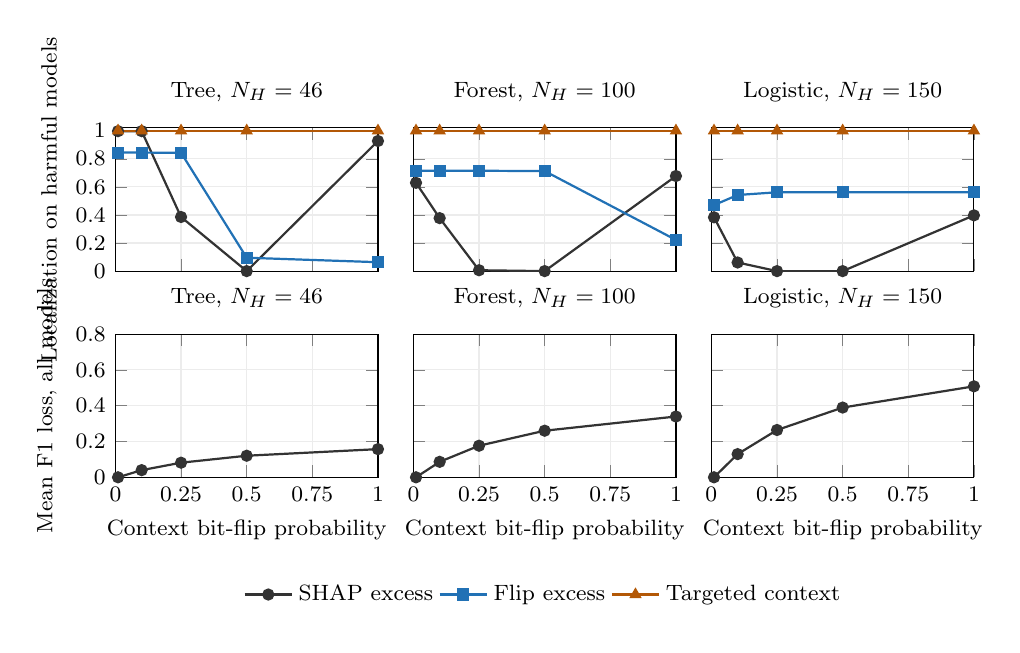
\begin{tikzpicture}
\begin{groupplot}[group style={group size=3 by 2,horizontal sep=0.45cm,vertical sep=0.8cm},
scale only axis,width=0.275\textwidth,height=0.15\textwidth,xmin=0,xmax=1,xtick={0,0.25,0.5,0.75,1},
tick label style={font=\footnotesize,/pgf/number format/fixed},label style={font=\footnotesize},title style={font=\footnotesize},
grid=major,grid style={gray!15},legend columns=3,legend style={font=\footnotesize,draw=none},every axis plot/.append style={line width=0.8pt,mark size=1.8pt}]
\nextgroupplot[title={Tree, $N_H=46$},ymin=0,ymax=1.02,ylabel={Localization on harmful models},xticklabels=\empty,legend to name=harm-legend]
\addplot+[color=black!80,mark=*,mark options={fill=black!80}] coordinates {(0.01,0.99684782608695643) (0.10000000000000001,0.99684782608695643) (0.25,0.38543478260869574) (0.5,0) (1,0.92673913043478262)};
\addlegendentry{SHAP excess}
\addplot+[color=auditblue,mark=square*,mark options={fill=auditblue}] coordinates {(0.01,0.84413043478260863) (0.10000000000000001,0.84413043478260863) (0.25,0.84293478260869559) (0.5,0.095326086956521741) (1,0.063478260869565206)};
\addlegendentry{Flip excess}
\addplot+[color=auditorange,mark=triangle*,mark options={fill=auditorange}] coordinates {(0.01,1) (0.10000000000000001,1) (0.25,1) (0.5,1) (1,1)};
\addlegendentry{Targeted context}
\nextgroupplot[title={Forest, $N_H=100$},ymin=0,ymax=1.02,yticklabels=\empty,xticklabels=\empty]
\addplot+[color=black!80,mark=*,mark options={fill=black!80}] coordinates {(0.01,0.62879999999999991) (0.10000000000000001,0.37739999999999996) (0.25,0.0062000000000000006) (0.5,0) (1,0.67730000000000035)};
\addplot+[color=auditblue,mark=square*,mark options={fill=auditblue}] coordinates {(0.01,0.71465000000000001) (0.10000000000000001,0.71465000000000001) (0.25,0.71465000000000001) (0.5,0.71265000000000012) (1,0.22194999999999998)};
\addplot+[color=auditorange,mark=triangle*,mark options={fill=auditorange}] coordinates {(0.01,1) (0.10000000000000001,1) (0.25,1) (0.5,1) (1,1)};
\nextgroupplot[title={Logistic, $N_H=150$},ymin=0,ymax=1.02,yticklabels=\empty,xticklabels=\empty]
\addplot+[color=black!80,mark=*,mark options={fill=black!80}] coordinates {(0.01,0.38329999999999997) (0.10000000000000001,0.061466666666666669) (0.25,0) (0.5,0) (1,0.39706666666666657)};
\addplot+[color=auditblue,mark=square*,mark options={fill=auditblue}] coordinates {(0.01,0.47023333333333334) (0.10000000000000001,0.5421999999999999) (0.25,0.56146666666666667) (0.5,0.56216666666666659) (1,0.56216666666666659)};
\addplot+[color=auditorange,mark=triangle*,mark options={fill=auditorange}] coordinates {(0.01,1) (0.10000000000000001,1) (0.25,1) (0.5,1) (1,1)};
\nextgroupplot[title={Tree, $N_H=46$},ymin=0,ymax=0.8,ylabel={Mean F1 loss, all models},xlabel={Context bit-flip probability}]
\addplot+[color=black!80,mark=*,mark options={fill=black!80}] coordinates {(0.01,0) (0.10000000000000001,0.039986261088843122) (0.25,0.081641904855032366) (0.5,0.12050965307934125) (1,0.15736954445100942)};
\nextgroupplot[title={Forest, $N_H=100$},ymin=0,ymax=0.8,yticklabels=\empty,xlabel={Context bit-flip probability}]
\addplot+[color=black!80,mark=*,mark options={fill=black!80}] coordinates {(0.01,0) (0.10000000000000001,0.086486931113268037) (0.25,0.17645176712867855) (0.5,0.26028364984520097) (1,0.33964327050237142)};
\nextgroupplot[title={Logistic, $N_H=150$},ymin=0,ymax=0.8,yticklabels=\empty,xlabel={Context bit-flip probability}]
\addplot+[color=black!80,mark=*,mark options={fill=black!80}] coordinates {(0.01,0) (0.10000000000000001,0.12955120406185197) (0.25,0.26424326465704007) (0.5,0.3896380302076049) (1,0.50822588460198193)};
\end{groupplot}
\node[anchor=north] at ([yshift=-1.1cm]group c2r2.south) {\pgfplotslegendfromname{harm-legend}};
\end{tikzpicture}

\caption{Fixed-candidate transfer at $n=10{,}000$. Top: localization on models losing at least 0.05 F1 under independent context. Bottom: mean loss over all 200 models. The targeted test knows $C$. Nominal fixed-function sizes coincide; independent-model warning rates need not.}
\label{fig:transfer-harm}
\end{figure*}

The flip-excess baseline retains 9.5\%, 71.3\%, and 56.2\% localization on the corresponding harmful subsets after shift. The targeted context test detects every harmful model but also warns on all no-harm forest and logistic candidates. It therefore separates input use from invariance, not harmless from harmful use. Fixed-bin SHAP also warns before shift on 32.6\% of no-harm forests and 5.6\% of no-harm logistic candidates.

At $n=10{,}000$, composite calibration does not repair the score's target: SHAP localization remains zero after context independence. For forests, composite global SHAP has 64.2\% pre-shift localization on harmful models and 0.4\% on no-harm models; fixed composite bins raise the latter to 33.8\%. Extra sensitivity to context is not necessarily extra specificity to transfer harm.

\subsection{Sensitivity at Matched Population Size}
\Cref{tab:matched-population} removes the different acceptable-model warning frequencies from the sensitivity comparison. At matched 5\% empirical size, post-shift SHAP localization is zero on the harmful $n=10{,}000$ subsets under both global and fixed-bin population ranks. Flip excess retains 8.4\%, 43.4\%, and 24.3\% with fixed bins; global values are 8.1\%, 47.0\%, and 20.7\%. The paired bootstrap intervals for these shifted differences exclude zero within the observed populations. Before shift, SHAP localizes more harmful trees than flip excess, so the comparison does not establish uniform score dominance.

\begin{table*}[t]
\centering
\caption{Localization (\%) at retrospectively matched 5\% empirical acceptable-model warnings, $n=10{,}000$. Harm-positive counts: 46/100/150 (tree/forest/logistic). Shifted difference is flip minus SHAP, in percentage points; intervals resample calibration pairs and evaluated cases. Zero observed localization is not a population power bound.}
\label{tab:matched-population}
\footnotesize
\begin{tabular}{llrrrrl}
\toprule
Learner & Calibration & SHAP, intact & Flip, intact & SHAP, shifted & Flip, shifted & Shifted difference [95\% interval] \\
\midrule
Tree & Global & 100.0 & 78.1 & 0.0 & 8.1 & 8.1 [5.2, 11.8] \\
Tree & Fixed bins & 99.7 & 72.8 & 0.0 & 8.4 & 8.4 [4.3, 13.1] \\
Forest & Global & 58.7 & 47.1 & 0.0 & 47.0 & 47.0 [36.2, 54.9] \\
Forest & Fixed bins & 65.5 & 43.5 & 0.0 & 43.4 & 43.4 [33.6, 54.3] \\
Logistic & Global & 7.9 & 17.1 & 0.0 & 20.7 & 20.7 [12.2, 31.8] \\
Logistic & Fixed bins & 34.9 & 20.1 & 0.0 & 24.3 & 24.3 [13.6, 36.3] \\
\bottomrule
\end{tabular}

\end{table*}

Matching reduces shifted forest flip localization from 71.3\% to 43.4\%. At a prospective nominal 5\% population cut, realized $n=10{,}000$ acceptable-model warnings range from 4.4--6.6\% for SHAP and 5.8--8.2\% for flip excess across the two partitions. The retrospective matched-rate comparison isolates sensitivity; it does not remove finite-bank error from the prospective rule.

\subsection{Overlap and Bin Choice}
\Cref{fig:overlap-score} shows that the null score varies with observed overlap. At $n=10{,}000$, the fixed bins explain 46.9--49.3\% of its target variance, whereas source quintiles explain only 7.5--8.3\%. Source tertiles put target batches in a single populated bin and reduce to the global rule in these runs. \Cref{tab:transfer-bins} shows the corresponding localization differences.

\begin{figure}[t]
\centering
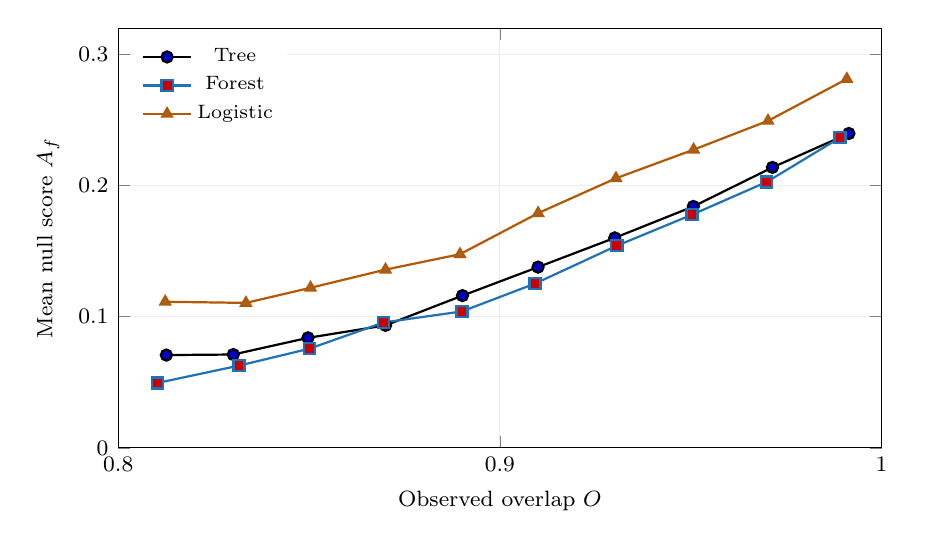
\begin{tikzpicture}
\begin{axis}[width=0.93\columnwidth,height=0.57\columnwidth,
xmin=0.8,xmax=1,xtick={0.8,0.9,1},ymin=0,ymax=0.32,grid=major,grid style={gray!15},
xlabel={Observed overlap $O$},ylabel={Mean null score $A_f$},
legend style={font=\scriptsize,at={(0.02,0.98)},anchor=north west,draw=none},
tick label style={font=\footnotesize,/pgf/number format/fixed},label style={font=\footnotesize}]
\addplot+[color=black,mark=*,line width=0.8pt] coordinates {(0.8126005148318366,0.070782833928559621) (0.83014585502408622,0.071209315571770973) (0.84970889628002144,0.083924499031962446) (0.87002688780748838,0.093443223853073298) (0.8901869253080712,0.11611985965636375) (0.90998279823456296,0.13786185301626536) (0.93007412003176848,0.16015641561634056) (0.95066127024303926,0.18409127618674093) (0.97140063748291461,0.21388699492222629) (0.99141899561271796,0.23974756828982696)};
\addlegendentry{Tree}
\addplot+[color=auditblue,mark=square*,line width=0.8pt] coordinates {(0.81020387291316409,0.049483548404018349) (0.83163297332729669,0.062737076897521282) (0.85004400083415921,0.075612892717808772) (0.86946993711680232,0.09560962542968679) (0.89005091942279602,0.1040690584874784) (0.90920523939467013,0.12529583559935689) (0.93064724407373467,0.15417736173449442) (0.95032483215036556,0.17781679468999562) (0.96990734765446418,0.20279653454244276) (0.98907957020173742,0.23654302766224064)};
\addlegendentry{Forest}
\addplot+[color=auditorange,mark=triangle*,line width=0.8pt] coordinates {(0.81230755017859158,0.11142666941911922) (0.8334489684776959,0.11055951094156777) (0.85037332167813551,0.12208415793194242) (0.87001570021759023,0.13593077645154092) (0.88953722732198792,0.14768622729906228) (0.91000784902351051,0.17899946868847411) (0.93040228502777644,0.20558012720915117) (0.95075434199266762,0.22741570367100022) (0.97023643431546969,0.24937918602042999) (0.99088130082424253,0.28130652525888417)};
\addlegendentry{Logistic}
\end{axis}
\end{tikzpicture}

\caption{Null score versus overlap for one $n=10{,}000$ reference per learner. Points average 1000 target-base batches within ten display intervals, distinct from calibration strata. Variance analysis uses all 200 references.}
\label{fig:overlap-score}
\end{figure}

\begin{table*}[t]
\centering
\caption{Bin sensitivity at $n=10{,}000$: target null variance explained by fixed bins and intact-law localization (\%) over 200 candidates. Source thirds/fifths use source-only edges; residual calibration is independent.}
\label{tab:transfer-bins}
\footnotesize
\begin{tabular}{lrrrrr}
\toprule
Learner & Variance explained & Global & Fixed bins & Source thirds & Source fifths \\
\midrule
Tree & 46.9 & 23.0 & 22.9 & 23.0 & 22.9 \\
Forest & 46.9 & 29.0 & 47.7 & 29.0 & 30.9 \\
Logistic & 49.3 & 8.5 & 30.1 & 8.5 & 11.4 \\
\bottomrule
\end{tabular}

\end{table*}

At $n=10{,}000$, fixed bins improve all-candidate localization by 18.8 percentage points for forests (case-bootstrap 95\% interval 15.2--22.0) and 21.6 for logistic models (18.8--24.4). Case-level sign tests in the twelve-test Holm family give adjusted $p=3.13\times10^{-9}$ and $5.88\times10^{-21}$. Tree localization instead decreases by 0.073 percentage points, a small effect despite adjusted $p=1.67\times10^{-6}$. Harmful tree cases already have almost saturated intact-law localization under the global threshold. Explained null variance alone cannot predict the gain: the alternative scores must also lie near the changed cut. Global all-candidate tree localization is 25.0\% at $n=1000$ and 23.0\% at $n=10{,}000$. The different training draws and harm-positive subsets prevent attributing that difference to audit size alone.

\subsection{Measured Attribution Audit}
\Cref{tab:cwru-audit} reports the actual descriptive audit. Under resonance, the largest outside-set excess is a broad-band feature for inner- and outer-race heads, but a different mechanism's harmonic for the ball head. Expected-set relevance alone changes little for the inner-race head. Broad-band share nevertheless increases for all three heads, most strongly for outer-race diagnosis. A band feature also maximizes the original inner-race head, so that feature type alone does not identify the injected resonance.

\begin{table*}[t]
\centering
\caption{CWRU diameter-held-out TreeSHAP audit. B/IR/OR: ball/inner/outer faults. Resonance and removed use the same confounded model, with/without its label-assigned response. Band share sums four broad-band features. These are descriptive scores without a calibrated mechanism-warning threshold.}
\label{tab:cwru-audit}
\footnotesize
\begin{tabular}{llrrrlr}
\toprule
Acquisition & Head & $R_m$ & $D_m$ & $S_m$ & Maximizing outside feature & Band share \\
\midrule
Original & B & 0.094 & 0.003 & 0.032 & log RMS & 0.165 \\
Original & IR & 0.372 & 0.029 & 0.036 & 4--6 kHz band & 0.189 \\
Original & OR & 0.388 & 0.015 & 0.016 & Kurtosis & 0.105 \\
Resonance & B & 0.060 & 0.007 & 0.048 & IR raw, first harmonic & 0.290 \\
Resonance & IR & 0.385 & 0.021 & 0.008 & 0--1 kHz band & 0.249 \\
Resonance & OR & 0.244 & -0.036 & 0.060 & 4--6 kHz band & 0.459 \\
Removed & B & 0.065 & 0.009 & 0.018 & OR raw, first harmonic & 0.316 \\
Removed & IR & 0.417 & 0.050 & 0.007 & 0--1 kHz band & 0.246 \\
Removed & OR & 0.282 & 0.028 & 0.051 & 0--1 kHz band & 0.390 \\
\bottomrule
\end{tabular}

\end{table*}

Original diagnosis F1 is 0.611. The injected information yields F1 0.886, falling to 0.313 after removal. The 0.573 paired drop gives exact nine-group swap $p=0.0625$; empirical group-bootstrap percentiles are 0.243--0.867. Only five groups change predictions. These finite-inventory results support acquisition-sensitivity investigation, but the ball-head maximizer misses the injected band information.

\subsection{Prospective Continuous-Process Audit}
\Cref{tab:dtu-prospective} exercises calibration on distinct fitted models and whole simulation packets. Unaltered fits give 0/60 SHAP warnings (exact 95\% interval 0--5.96\%) and 1/60 response warnings (0.042--8.94\%). These conditional-on-bank frequencies do not establish equal population size. The separate 95\% calibration-bank tolerance upper bound is 8.92\%; the marginal rank guarantee averages over bank randomness.

Both scores localize the constructed bias after removal or reversal; SHAP also localizes all matched cases. Removing the bias lowers mean F1 by 0.301. Because fault prevalence is 75\%, an all-positive predictor has F1 0.857 and balanced accuracy 0.5: the unaltered model improves balanced accuracy, not F1, against that baseline. The matched gain is injected information. This test demonstrates a feasible prospective audit under a stated training/simulation law, not verified causal alignment or field acquisition independence.

\begin{table}[t]
\centering
\caption{Prospective DTU process audit. W/L gives warning/localization counts out of 60; localization identifies Compressor Work. BA is balanced accuracy. Thresholds are frozen before evaluation, without empirical size matching.}
\label{tab:dtu-prospective}
\footnotesize
\begin{tabular}{lrrrr}
\toprule
Condition & F1 & BA & SHAP W/L & Response W/L \\
\midrule
Unaltered & 0.746 & 0.763 & 0/0 & 1/0 \\
Biased, matched & 0.965 & 0.939 & 60/60 & 39/38 \\
Bias removed & 0.665 & 0.717 & 60/60 & 60/60 \\
Bias reversed & 0.632 & 0.699 & 60/60 & 60/60 \\
\bottomrule
\end{tabular}

\end{table}

\subsection{Field Diagnosis and Comparison Support}
\Cref{tab:sca-field} reports case-held-out field predictions. The 21-feature model has F1 0.299 and healthy prediction false-positive rate 12.4\%. Pooled cross-fitted expected shares are 0.161/0.173/0.371 for inner/ball/outer faults, supplied by five/one/four cases. Each held-out case contains only one recorded fault type, so within-case $D_m,S_m$ comparisons are unavailable. Pooling fold models introduces fitting variation into a mechanism-specificity contrast. Even before training, these cases permit at most one disjoint three-type comparison batch. Unsupported calibrated claims require abstention.

\begin{table}[t]
\centering
\caption{SCA case-held-out predictions, with cases weighted equally. FPR is prediction error, distinct from explanation-warning size. Case 11 uses 38 test-period measurements and the frozen ensemble.}
\label{tab:sca-field}
\footnotesize
\begin{tabular}{lrrrr}
\toprule
View & F1 & Healthy FPR & Recall & Case 11 FPR \\
\midrule
12 anchors & 0.300 & 0.134 & 0.298 & 0.000 \\
21 features & 0.299 & 0.124 & 0.287 & 0.000 \\
\bottomrule
\end{tabular}

\end{table}

\section{Experimental Analysis}
\label{sec:analysis}
\subsection{Reference Transfer and Error Targets}
A fixed-reference rank guarantee does not imply low warning rates for another model with the same decisions. Mechanism-only probability tables differ after fitting, and their normalized attribution scores differ accordingly. A composite reference addresses that variation only when a credible model-generating population can be specified. It changes the null from one function to one training population; it does not remove the need to justify alignment.

Case-bootstrap intervals condition on the realized bank; order-statistic bounds quantify bank randomness. Matched-rate analysis resamples both. Non-rejection of a 5\% frequency is not a validity argument.

\subsection{Why Harm Can Escape Localization}
The SHAP statistic asks whether an outside feature has unusually concentrated attribution on one mechanism's failure rows. Context independence can remove that concentration while leaving the predictor strongly dependent on context. Moreover, $S_m$ compares only recorded failure groups, whereas F1 loss includes false positives on normal rows. At $n=10{,}000$, aggregate false-positive rates under independent context are 11.5\%, 25.0\%, and 37.5\% for tree, forest, and logistic candidates; false-negative rates stay below 0.4\%. The score misses harm occurring largely outside its comparison cohorts. Localization can reappear under reversal while F1 loss increases (\cref{fig:transfer-harm}); it is not a monotone measure of harm.

A direct response test is therefore an essential comparator. The targeted baseline exposes context use cheaply, including use with no specified harm. The flip-excess baseline preserves some shift sensitivity but inherits reference-transfer problems. The evidence supports neither a general SHAP sensitivity advantage nor a rule that every redundant input should trigger an engineering alarm.

\subsection{Calibration and Compute Requirements}
For a finite $\alpha$ rank cut, a calibration stratum needs at least
\begin{equation}
 B_{\min}(\alpha)=\lceil1/\alpha\rceil-1
\end{equation}
independent units. Thus $K$ base strata plus one residual-calibration bank require at least $(K+1)B_{\min}$ units to make every cut finite: 76 at 5\% for three strata, before evaluation. This is only a rank-resolution minimum. Population-reference calibration uses independent fitted-model/batch pairs; repeating batches from one fitted function cannot replace those model draws.

Boolean compression costs $O(Bd4^d)$ arithmetic for $B$ batches after forming counts in $O(Bnd)$ time; it is exponential in feature count $d$. Sampled interventional SHAP with $n$ rows, $b$ backgrounds, and $\ell$ coalitions needs roughly $nb\ell$ model evaluations. TreeSHAP exploits tree structure, but background size still affects cost. In CWRU, 576 window explanations per fold with 96 backgrounds take \cwruShapRuntime{} seconds on \cwruHardware{} using SHAP \cwruShapVersion{}. The process experiment takes \dtuModelRuntime{} seconds with four workers for 220 fits, 43,520 explanations (32 backgrounds), and direct responses; source extraction takes \dtuSourceRuntime{} seconds. A prediction-equivalent float32 split encoding avoids threshold-rounding errors; every attribution passes unchanged $10^{-6}$ additivity checks, and all earlier attributions are exactly unchanged. Compute does not create acquisition units.

For $M_{\rm mech}$ mechanisms, stratifying every overlap pair into $K$ categories could create $K^{M_{\rm mech}(M_{\rm mech}-1)/2}$ cells. The present one-pair conditioning rule offers no remedy for that support problem. Fewer prespecified summaries or a conditional method require a new support and calibration assessment.

\subsection{Limitations and Reproducibility}
The controlled mechanisms and acceptable training populations are supplied definitions, not industrial causal truth. DTU tests two simulated disturbances and a deliberately strong label-assigned bias, with partial component maps and publisher-described replicate assumptions. Its prospective result does not establish mild-confound sensitivity, arbitrary-model coverage, or new-plant transfer. Context shifts are constructed, and harm-conditioned summaries use realized evaluation loss. Calibration inference is tied to the stated function or training law. Source-quantile sensitivity shows that the fixed bins exploit useful generator structure rather than a universally transferable partition.

CWRU has few bearing states, one rig, no healthy class, and partial maps. It supplies at most two matched or eleven pooled calibration batches after test reservation, without a justified reference. SCA adds healthy field records but unverified session independence. A separate physical-chamber source audit authenticates 57 intervention records; 32 replay their published schedules. All 627 intervention/channel pairs are assessed, with unresolved relationships retained. Positive intervention evidence does not certify excluded effects or independent new-machine acquisitions. None of these data supports an exhaustive causal map or calibrated industrial mechanism-warning claim.

The research is exploratory; dated protocols distinguish settings fixed before each follow-up outcome from subsequent analyses. The primary case-level sign-test family has twelve Holm-adjusted comparisons; other analyses are descriptive. Source hashes, signed attributions, probability tables, count vectors and verifier scripts are released. A single command, \texttt{reproduce\_reference\_study.sh}, reproduces the focused studies and paper. The work evaluates tabular explanation audits and their requirements, rather than temporal attribution or a large-scale monitoring system.

\section{Conclusion}
Reference design determines the scope of a mechanism-level SHAP warning. Overlap produces outside excess; acceptable refits exceed fixed-function thresholds; harmful reliance may escape localization. Calibration over independent training outcomes supports a specified population. The prospective process audit demonstrates feasibility under that law; field studies delimit its physical interpretation. Engineers should report the reference population, independent units, comparison cohorts, and supported action.

\section{Future Work}
\subsection{Industrial Validation}
Reserve independent healthy/faulty acquisitions and inspection-based mechanism information before fitting. A physically justified reference population would enable field transfer-warning assessment.

\subsection{Harm-Sensitive Scores and Calibration}
Include normal-row errors and maintenance loss; compare continuous conditional calibration and realistic acquisition shifts against direct response tests at equal data budgets. Temporal attribution and deployment need separate evaluations.

\section*{Acknowledgment}
AI systems assisted manuscript and analysis-code drafting, including Claude (Anthropic) and Codex (OpenAI). The authors are responsible for the scientific claims and verification. Code, protocols, results, and verification scripts are available at \url{https://github.com/kowshik24/glowing-broccoli}.
\bibliographystyle{IEEEtran}
\bibliography{refs}
\end{document}
